\documentclass[10pt, red]{beamer}
\usetheme{JuanLesPins}
\usepackage[english]{babel}
\usepackage[latin1]{inputenc} 
\setbeamercovered{transparent}


\title[CudaQCAD]{A Parallel Version of the Mina's Quantum Cellular Automata Designer}

\author{Riccardo Cattaneo, Giuseppe Chindemi}

\institute{
  Politecnico di Milano\\
  HPPS
}

\date{June 22 2010}

\pgfdeclareimage[height=0.5cm]{logo}{img/polimi}
\logo{\pgfuseimage{logo}}


\begin{document}

\begin{frame}
  \titlepage
\end{frame}


\section{Introduction}
	\begin{frame}{1}
	\end{frame}


\section{QCADesigner}
	\begin{frame}{2}
	\end{frame}


\section{Nvidia Cuda}

	\begin{frame}{Cuda Overview}
		What is Cuda?		
		\begin{itemize}
			\item It is a software layer that allow programmers to exploit the capability of Nvidia GPUs as general purpose processors.
		\end{itemize}
		Why Cuda for QCAD?
		\begin{itemize}
			\item Because QCA are parrallel by nature.
			\item Because GPUs are good in arithmeric.
			\item Because GPUs offer the lower price per core.
		\end{itemize}
	\end{frame}

	\begin{frame}{GPU Logical Organization and Programming Model}
		\begin{columns}
    		\column{.4\textwidth}
		 	\begin{figure}
				\centering
				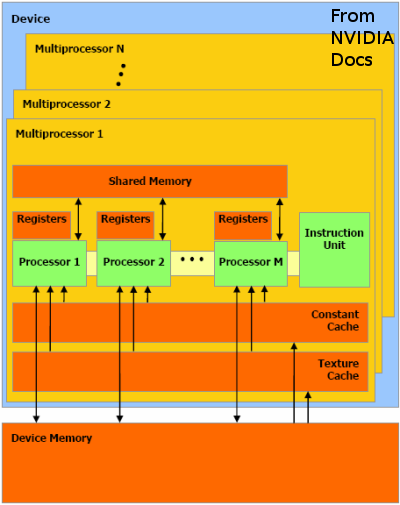
\includegraphics[width=\textwidth, height=0.6\textheight]{img/HWModel}
				\caption{Cuda GPUs: A MIMD Array of SIMD processors}
		 	\end{figure} 
			\column{.4\textwidth}
			\begin{figure}
				\centering
				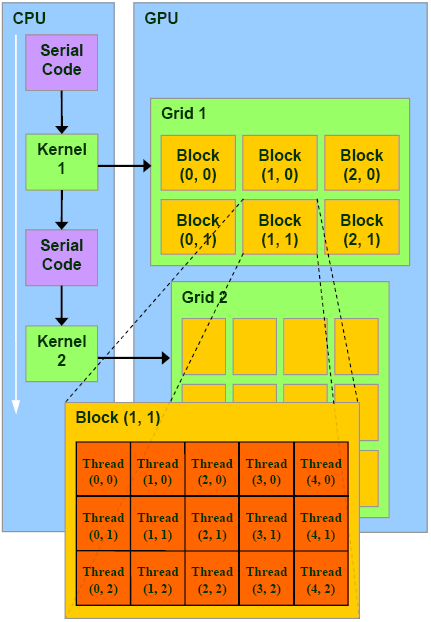
\includegraphics[width=\textwidth, height=0.6\textheight]{img/nVidiaExecutionModel}
				\caption{CUDA GPUs: Eterogeneous Programming}
			\end{figure}
		\end{columns}
	\end{frame}


\section{Implementation}
	\begin{frame}{3}
	\end{frame}


\section{Results}

	\begin{frame}{Tests Description}
		The "Lucifero" Workstation
		\begin{description}
			\item[CPU] Intel Xeon E5345
			\item[GPU] Nvidia Testa C1060
		\end{description}
		Which Tests?
		\begin{description}
			\item[Test 1] QCAD vs CudaQCAD
			\item[Test 2] Memory Transfert Rate
			\item[Test 3] GPU Occupancy
		\end{description}
	\end{frame}

	\begin{frame}{Test 1: QCAD vs CudaQCAD}
	 	\begin{figure}
			\centering
			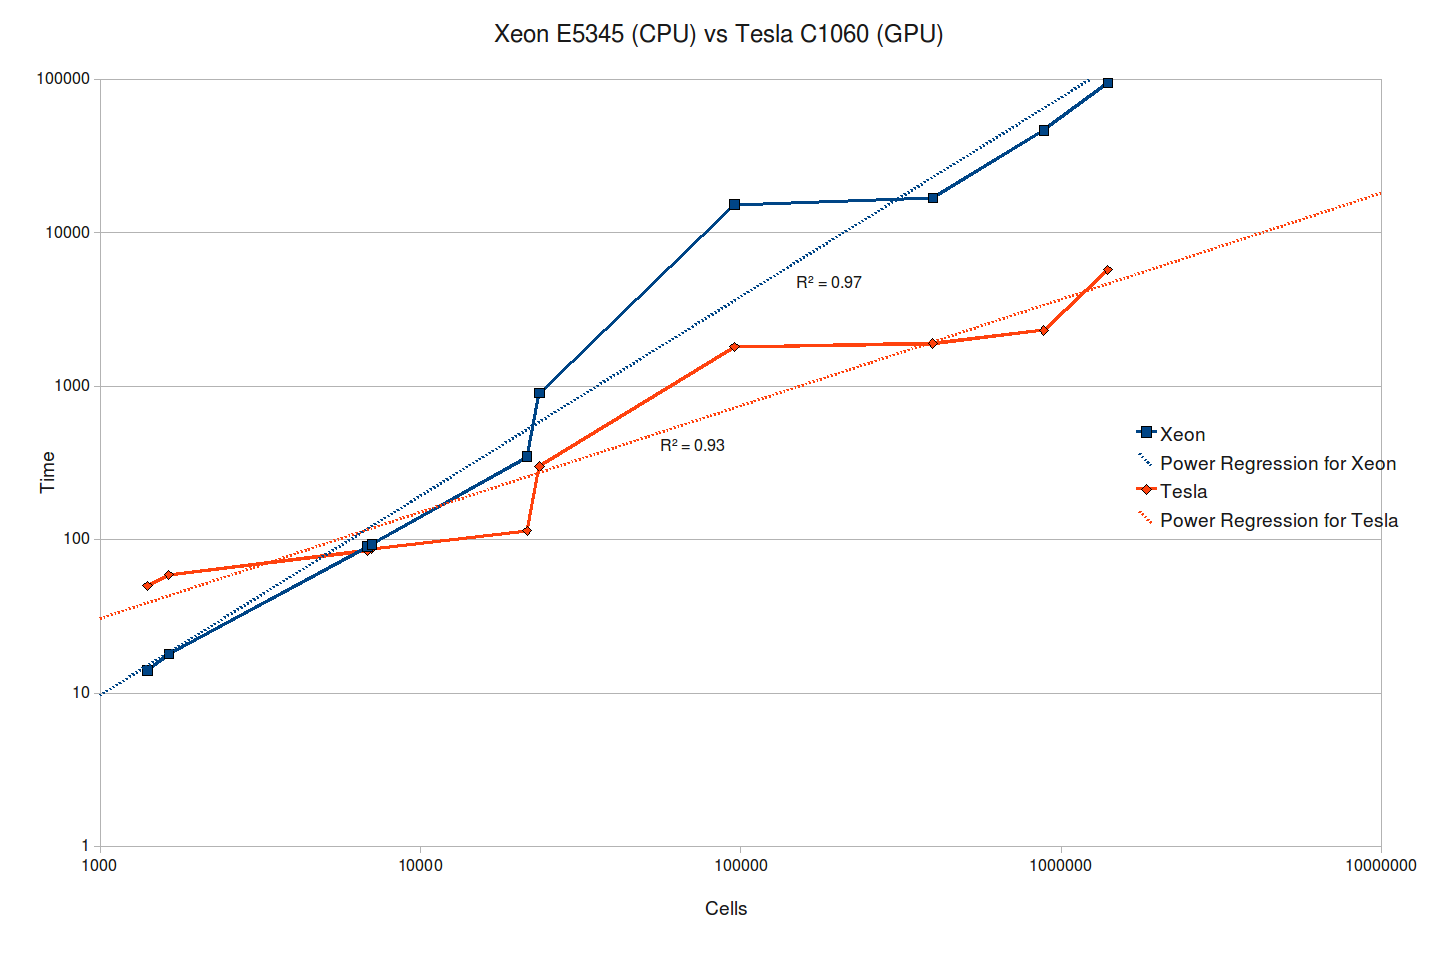
\includegraphics[width=\textwidth]{img/xeonvstesla}
	 	\end{figure} 
	\end{frame}

	\begin{frame}{Test 1: QCAD vs CudaQCAD}
	 	\begin{figure}
			\centering
			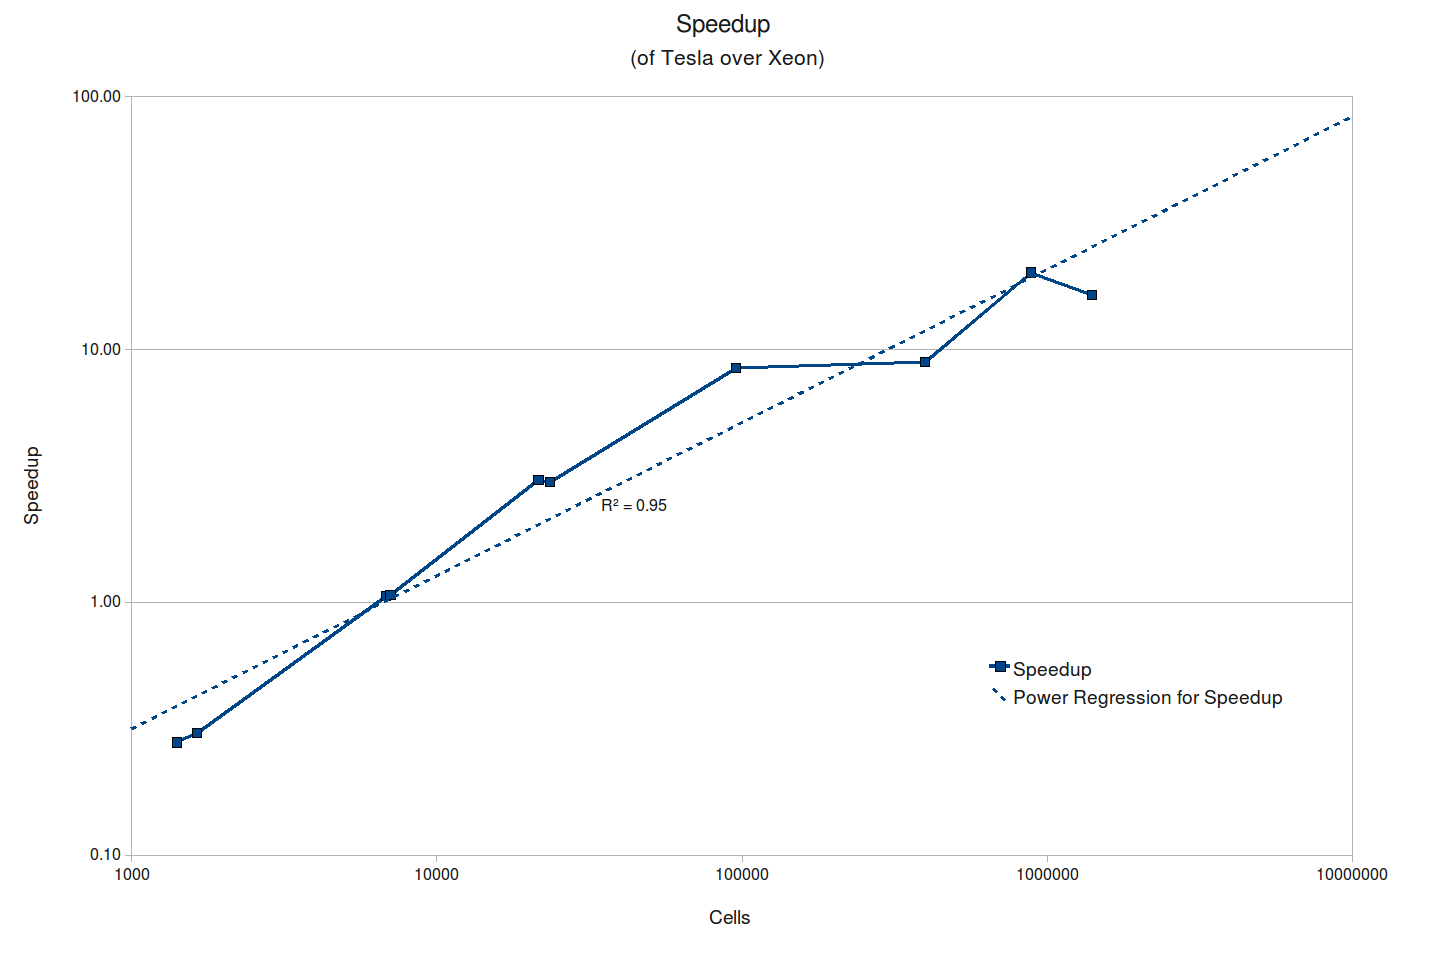
\includegraphics[width=\textwidth]{img/speedup}
	 	\end{figure} 
	\end{frame}

	\begin{frame}{Test 2: Memory Transfert Rate}
	 	\begin{figure}
			\centering
			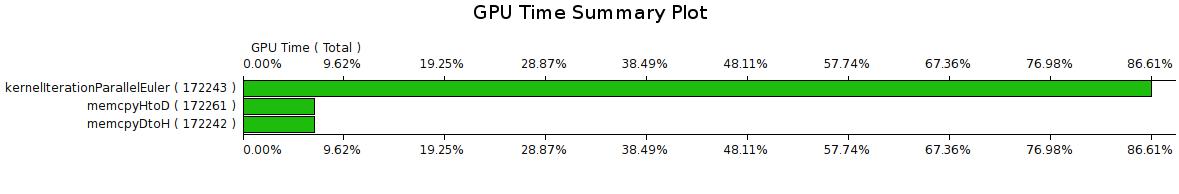
\includegraphics[width=\textwidth]{img/GPUTimeSummaryPlotNAND}
			\caption{Memory Tranfer for NAND circuit (1642 cells)}
	 	\end{figure} 
		\begin{figure}
			\centering
			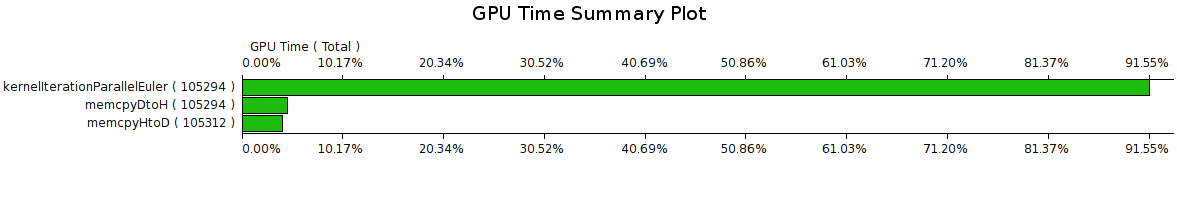
\includegraphics[width=\textwidth]{img/GPUTimeSummaryPlotMUX42}
			\caption{Memory transfers for MUX42 circuit (21551 cells)}
		\end{figure}
	\end{frame}

	\begin{frame}{Test 3: GPU Occupancy}
	 	\begin{figure}
			\centering
			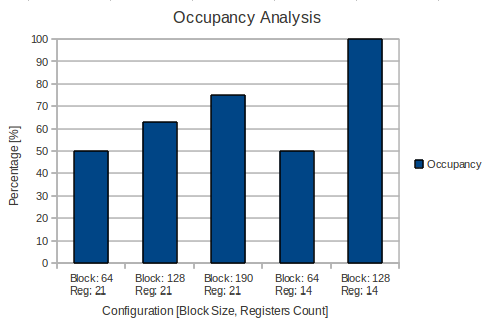
\includegraphics[width=\textwidth]{img/OccupancyAnalysis}
	 	\end{figure} 
	\end{frame}

	\begin{frame}{Conclusions}
	\end{frame}


\end{document}
